\section{Feature 132}
The feature was described as "As a user, I would like to be able to switch between guardian and citizen mode so that I can only access the parts of the system that I should be able to" alongside the description \gls{PO} had set two requirements:

\begin{itemize}
  \item The system stores whether the user is currently in citizen or guardian mode
  \item A guardian can see the add new activities function, but a citizen cannot
\end{itemize}

This feature was first to implement by introducing a new stream to the weekplan \gls{bloc} which we then could use a stream builder in the \gls{ui} to determine how the screen should render out, i.e., having the guardian functionality or citizen functionality.

\begin{figure}[h]
    \centering
    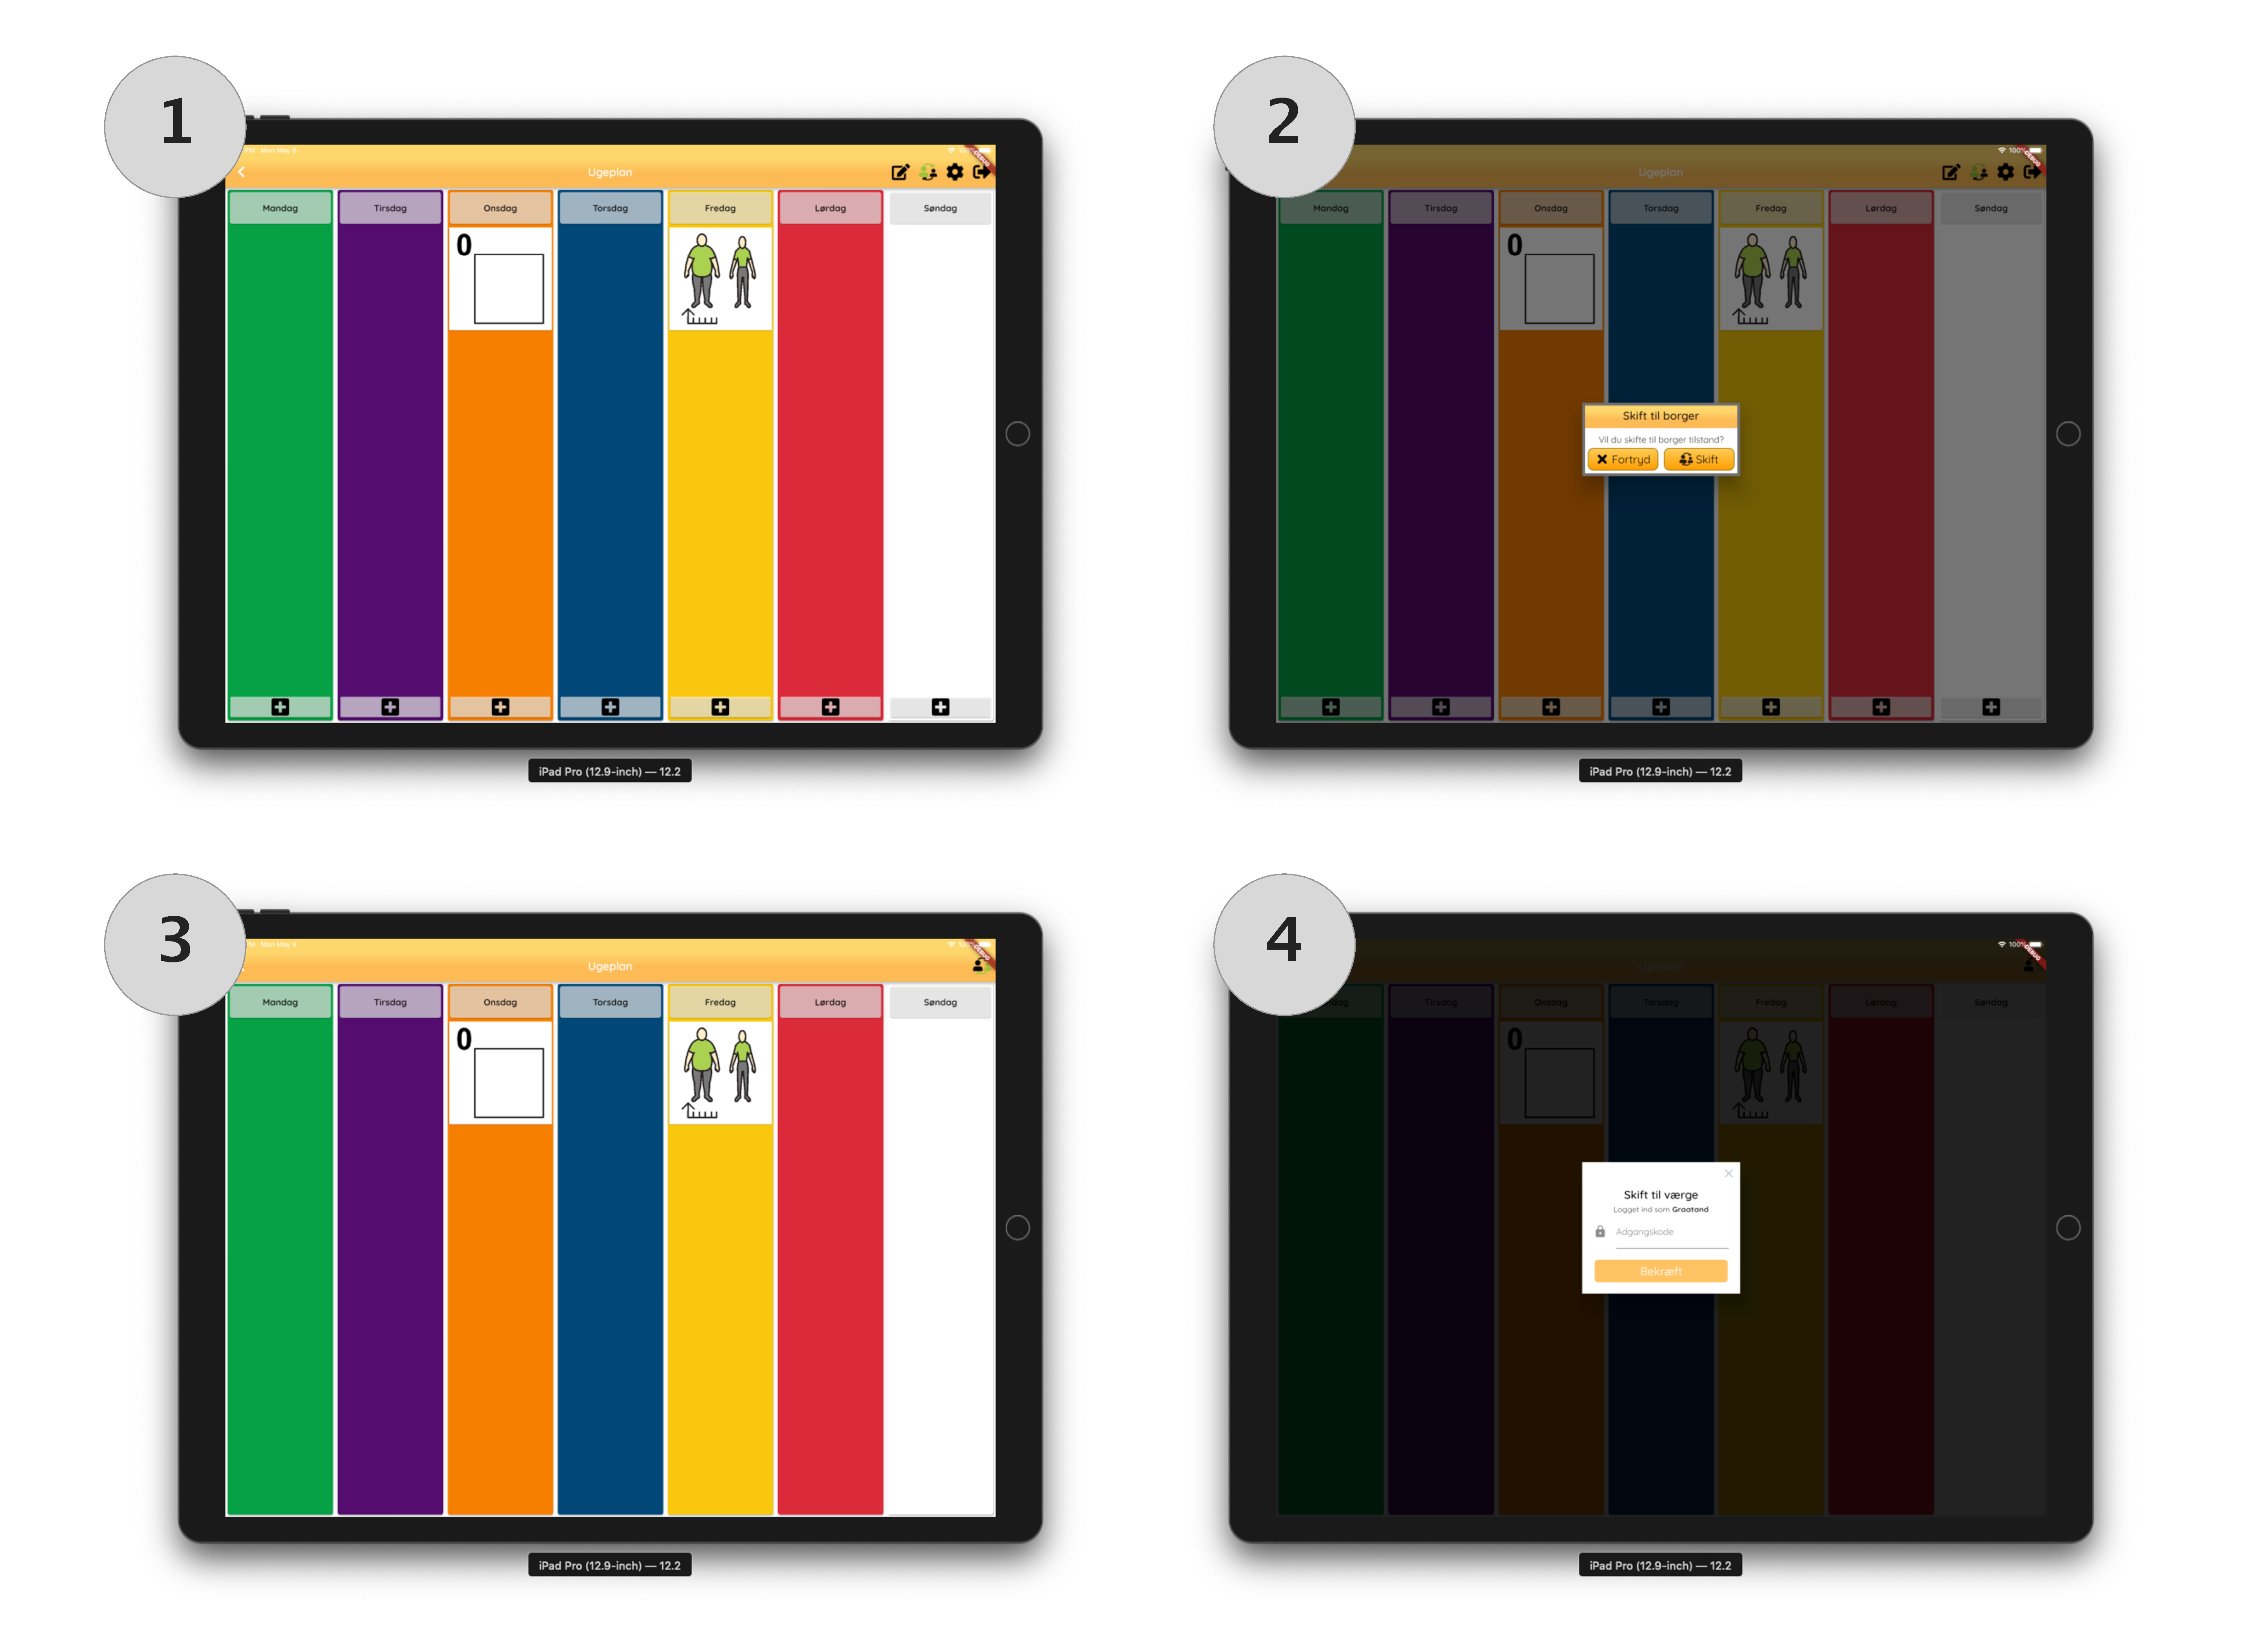
\includegraphics[width=0.8\textwidth]{figures/feature_132.pdf}
    \caption{A illustration of the final result after implementing feature 132}
    \label{fig:feature132}
\end{figure}

When clicking the "switch to x"-icon (where x denotes either guardian or citizen), it would then switch the mode that is emitted on the new stream. \gls{PO} informed us that when clicking the icon "switch to citizen-mode" the app should prompt the user with a "are you sure"-dialog which we then implemented.

While we developed the feature, other guardian-only-functionality were introduced into the product, and our feature had to handle the availability of those functionalities also. Accommodating the new functionalities lead us to believe that placing the responsibility of managing whether a user is guardian or citizen did not belong to the weekplan \gls{bloc} but rather the authentication \gls{bloc}. Therefore we moved it and again used the Flutter stream-builder widget to handle the rendering of the screen.

All in all, the implementation allows developers to use a stream builder widget and in there do an if-else statement to handle functionality for the citizen mode and guardian mode, which offers a clean and comprehensive way to handle the restriction of features.